\documentclass{beamer}

\usepackage{framed}
\usepackage{graphicx}

\begin{document}
%====================================%
\begin{frame}[fragile]
\frametitle{Seaborn Workshop}
\large

\noindent \textbf{Choosing color palettes}
\begin{itemize}
\item Color is more important than other aspects of figure style because color can reveal patterns in the data if used effectively or hide those patterns if used poorly. 
\item There are a number of great resources to learn about good techniques for using color in visualizations, I am partial to this series of blog posts from Rob Simmon and this more technical paper. 
\item The matplotlib docs also now have a nice tutorial that illustrates some of the perceptual properties of the built in colormaps.
\end{itemize}

\end{frame}
%====================================%
\begin{frame}[fragile]
\frametitle{Seaborn Workshop}
\large
Seaborn makes it easy to select and use color palettes that are suited to the kind of data you are working with and the goals you have in visualizing it.
{
	\Large
\begin{framed}
\begin{verbatim}
%matplotlib inline
import numpy as np
import seaborn as sns
import matplotlib.pyplot as plt
sns.set(rc={"figure.figsize": (6, 6)})
np.random.seed(sum(map(ord, "palettes")))
\end{verbatim}
\end{framed}
}
\end{frame}
\section{Building color palettes with \texttt{color\_palette()}}
%====================================%
\begin{frame}[fragile]
\frametitle{Seaborn Workshop}
\Large

\textbf{Building color palettes with \texttt{color\_palette()}}\\
\begin{itemize}
\item The most important function for working with discrete color palettes is \texttt{color\_palette()}.
\item  This function provides an interface to many (though not all) of the possible ways you can generate colors in seaborn.
\item it is used internally by any function that has a palette argument (and in some cases for a color argument when multiple colors are needed).
\end{itemize}

\end{frame}
%====================================%
\begin{frame}[fragile]
	\frametitle{Seaborn Workshop}
	\large
	
\begin{itemize}
\item \texttt{color\_palette()} will accept the name of any seaborn palette or matplotlib colormap (except jet, which you should never use). 
\item It can also take a list of colors specified in any valid matplotlib format (RGB tuples, hex color codes, or HTML color names). \item The return value is always a list of RGB tuples.
\end{itemize}

\end{frame}
%====================================%
\begin{frame}[fragile]
\frametitle{Seaborn Workshop}
\Large
\begin{itemize}
\item Finally, calling \texttt{color\_palette()} with no arguments will return the current default color cycle.

\item A corresponding function, set\_palette(), takes the same arguments and will set the default color cycle for all plots. 
\item You can also use \texttt{color\_palette()} in a with statement to temporarily change the default palette (see below).
\end{itemize}

\end{frame}
%====================================%
\begin{frame}[fragile]
	\frametitle{Seaborn Workshop}
	\Large
\begin{itemize}
\item It is generally not possible to know what kind of color palette or colormap is best for a set of data without knowing about the characteristics of the data.
\item Following that, we’ll break up the different ways to use \texttt{color\_palette()} and other seaborn palette functions by the three general kinds of color palettes:
\end{itemize}
{ \Large \begin{enumerate}
\item qualitative, 
\item sequential, 
\item diverging.
\end{enumerate}
}

\end{frame}
%====================================%
\begin{frame}[fragile]
\frametitle{Seaborn Workshop}
\large
\noindent \textbf{Qualitative color palettes}\\
\begin{itemize}
\item Qualitative (or categorical) palettes are best when you want to distinguish discrete chunks of data that do not have an inherent ordering.

\item When importing seaborn, the default color cycle is changed to a set of six colors that evoke the standard matplotlib color cycle while aiming to be a bit more pleasing to look at.
\end{itemize}

\end{frame}
%====================================%
\begin{frame}[fragile]
	\frametitle{Seaborn Workshop}
	\large
\begin{verbatim}
current_palette = sns.color_palette()
sns.palplot(current_palette)
\end{verbatim}
\begin{figure}
\centering

\includegraphics[width=0.7\linewidth]{images/color_palettes_8_0}
\end{figure}

There are six variations of the default theme, called deep, muted, pastel, bright, dark, and colorblind.
\end{frame}
%====================================%
\begin{frame}[fragile]
\frametitle{Seaborn Workshop}
\large
\noindent \textbf{Using circular color systems}
\begin{itemize}
\item When you have more than six categories to distinguish, the easiest thing is to draw evenly-spaced colors in a circular color space (such that the hue changes which keeping the brightness and saturation constant). 
\item This is what most seaborn functions default to when they need to use more colors than are currently set in the default color cycle.
\end{itemize}

\end{frame}
%====================================%
\begin{frame}[fragile]
	\frametitle{Seaborn Workshop}
	\large
The most common way to do this uses the \texttt{hls} color space, which is a simple transformation of RGB values.

\begin{verbatim}
sns.palplot(sns.color_palette("hls", 8))
\end{verbatim}
\begin{figure}
\centering

\includegraphics[width=0.9\linewidth]{images/color_palettes_10_0}


\end{figure}


\end{frame}
%====================================%
\begin{frame}[fragile]
	\frametitle{Seaborn Workshop}
	\large
There is also the \texttt{hls\_palette()} function that lets you control the lightness and saturation of the colors.
\begin{verbatim}
sns.palplot(sns.hls_palette(8, l=.3, s=.8))
\end{verbatim}
\begin{figure}
\centering

\includegraphics[width=0.9\linewidth]{images/color_palettes_12_0}
\end{figure}

\end{frame}
%====================================%
\begin{frame}[fragile]
\frametitle{Seaborn Workshop}
\large
\begin{itemize}
\item However, because of the way the human visual system works, colors that are even “intensity” in terms of their RGB levels won’t necessarily look equally intense.
\item  We perceive yellows and greens as relatively brighter and blues as relatively darker, which can be a problem when aiming for uniformity with the \texttt{hls} system.
\end{itemize}

\end{frame}
	%====================================%
	\begin{frame}[fragile]
		\frametitle{Seaborn Workshop}
		\large
		
		To remedy this, seaborn provides an interface to the husl system, which also makes it easy to select evenly spaced hues while keeping the apparent brightness and saturation much more uniform.
		\begin{verbatim}
		sns.palplot(sns.color_palette("husl", 8))
		\end{verbatim}
		
		\begin{figure}
			\centering
			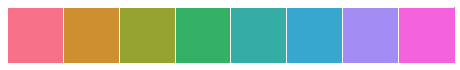
\includegraphics[width=0.7\linewidth]{images/color_palettes_14_0}
		\end{figure}
		
		There is similarly a function called \texttt{husl\_palette()} that provides a more flexible interface to this system.
	\end{frame}
	\section{Using categorical Color Brewer palettes}
	%====================================%
	\begin{frame}[fragile]
		\frametitle{Seaborn Workshop}
		\large
		\textbf{Using categorical Color Brewer palettes}
		\begin{itemize}
			\item Another source of visually pleasing categorical palettes comes from the \textbf{Color} \textbf{Brewer} tool (which also has sequential and diverging palettes, as we’ll see below). 
			\item These also exist as matplotlib colormaps, but they are not handled properly. 
			\item In seaborn, when you ask for a qualitative \textbf{Color} \textbf{Brewer} palette, you’ll always get the discrete colors, but this means that at a certain point they will begin to cycle.
		\end{itemize}
		
	\end{frame}
	%====================================%
	\begin{frame}[fragile]
		\frametitle{Seaborn Workshop}
		\large
		\begin{itemize}
			\item A nice feature of the \textbf{\textit{Color Brewer}} website is that it provides some guidance on which palettes are color blind safe. 
			\item There are a variety of [kinds](http://en.wikipedia.org/wiki/Color\_blindness) of color blindness, but the most common variant leads to difficulty distinguishing reds and greens.
			\item It’s generally a good idea to avoid using red and green for plot elements that need to be discriminated based on color.
		\end{itemize}
	\end{frame}
	%====================================%
	\begin{frame}[fragile]
		\frametitle{Seaborn Workshop}
		\large
		\begin{verbatim}
		sns.palplot(sns.color_palette("Paired"))
		\end{verbatim}
		
		\begin{figure}
			\centering
			
\includegraphics[width=0.7\linewidth]{images/color_palettes_16_0}
		\end{figure}
		\bigskip
		\begin{verbatim}
		sns.palplot(sns.color_palette("Set2", 10))
		\end{verbatim}
		\begin{figure}
			\centering
			
\includegraphics[width=0.7\linewidth]{images/color_palettes_17_0}
			
		\end{figure}
	\end{frame}
	%====================================%
	\begin{frame}[fragile]
		\frametitle{Seaborn Workshop}
		\large
		\begin{itemize}
			\item To help you choose palettes from the Color Brewer library, there is the \texttt{choose\_colorbrewer\_palette()} function.
			\item This function, which must be used in an IPython notebook, will launch an interactive widget that lets you browse the various options and tweak their parameters.
		\end{itemize}
		
	\end{frame}
	%====================================%
	\begin{frame}[fragile]
		\frametitle{Seaborn Workshop}
		\large
		
		Of course, you might just want to use a set of colors you particularly like together. Because \texttt{color\_palette()} accepts a list of colors, this is easy to do.
		\begin{verbatim}
		flatui = ["#9b59b6", "#3498db", "#95a5a6", "#e74c3c", "#34495e", "#2ecc71"]
		sns.palplot(sns.color_palette(flatui))
		\end{verbatim}
		\begin{figure}
			\centering
			
\includegraphics[width=0.7\linewidth]{images/color_palettes_19_0}
		\end{figure}
	\end{frame}
	\section{Using named colors from the xkcd color survey}
	
	%====================================%
	\begin{frame}[fragile]
		\frametitle{Seaborn Workshop}
		\large
		\noindent \textbf{xkcd}
		\begin{itemize}
			\item A while back, xkcd ran a crowdsourced effort to name random RGB colors. 
			\item This produced a set of 954 named colors, which you can now reference in seaborn using the \texttt{xkcd\_rgb} dictionary:
		\end{itemize}
		
	\end{frame}
	%====================================%
	\begin{frame}[fragile]
		\frametitle{Seaborn Workshop}
		\large
		\begin{verbatim}
		plt.plot([0, 1], [0, 1], sns.xkcd_rgb["pale red"], lw=3)
		plt.plot([0, 1], [0, 2], sns.xkcd_rgb["medium green"], lw=3)
		plt.plot([0, 1], [0, 3], sns.xkcd_rgb["denim blue"], lw=3);
		\end{verbatim}
		
		\begin{figure}
			\centering
			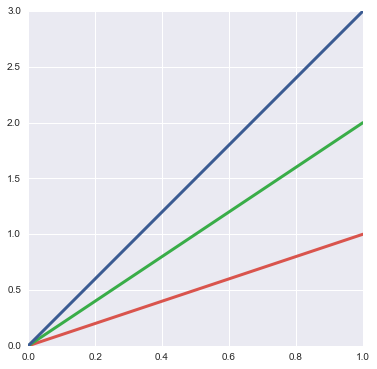
\includegraphics[width=0.55\linewidth]{images/color_palettes_21_0}
		\end{figure}
	\end{frame}
	%====================================%
	\begin{frame}[fragile]
		\frametitle{Seaborn Workshop}
		\large
		If you want to spend some time picking colors, this interactive visualization may be useful. In addition to pulling out single colors from the \texttt{xkcd\_rgb} dictionary, you can also pass a list of names to the \texttt{xkcd\_palette()} function.
		\begin{verbatim}
		
		colors = ["windows blue", "amber", "greyish", 
		          "faded green", "dusty purple"]
		          
		sns.palplot(sns.xkcd_palette(colors))
		\end{verbatim}
		
		\begin{figure}
			\centering
			
\includegraphics[width=0.7\linewidth]{images/color_palettes_23_0}
			
		\end{figure}
		
	\end{frame}
	

\section{Sequential color palettes}
%====================================%
\begin{frame}
	\frametitle{Seaborn Workshop}
	\large
	
	\textbf{Sequential color palettes}
	\begin{itemize}
		\item The second major class of color palettes is called “sequential”. 
		\item This kind of color mapping is appropriate when data range from relatively low or unintersting values to relatively high or interesting values. 
		\item Although there are cases where you will want discrete colors in a sequential palette, it’s more common to use them as a colormap in functions like \texttt{kdeplot()} or \texttt{corrplot()} (along with similar matplotlib functions).
	\end{itemize}
	
\end{frame}
%====================================%
\begin{frame}[fragile]
	
	\frametitle{Seaborn Workshop}
	\large
	\begin{itemize}
		\item It’s common to see colormaps like jet (or other rainbow palettes) used in this case, becuase the range of hues gives the impression of providing additional information about the data. 
		\item However, colormaps with large hue shifts tend to introduce discontinuities that don’t exist in the data, and our visual system isn’t able to naturally map the rainbow to quantitative distinctions like “high” or “low”. 
	\end{itemize}
\end{frame}
%====================================%
\begin{frame}[fragile]
	
	\frametitle{Seaborn Workshop}
	\large
	\begin{itemize}
		\item The result is that these visualizations end up being more like a puzzle, and they obscure patterns in the data rather than revealing them. 
		\item The jet palette is particularly bad because the brightest colors, yellow and cyan, are used for intermediate data values. This has the effect of emphasizing uninteresting (and arbitrary) values while demphasizing the extremes.
	\end{itemize}
\end{frame}
%====================================%
\begin{frame}[fragile]
	\frametitle{Seaborn Workshop}
	\large
	\begin{itemize}
		\item For sequential data, it’s better to use palettes that have at most a relatively subtle shift in hue accompanied by a large shift in brightness and saturation. 
		\item This approach will naturally draw the eye to the relatively important parts of the data.
	\end{itemize}
\end{frame}
%====================================%
\begin{frame}[fragile]
	\frametitle{Seaborn Workshop}
	\large
	\noindent \textbf{Color Brewer Palettes}\\
	The Color Brewer library has a great set of these palettes. They’re named after the dominant color (or colors) in the palette.
	
%\end{frame}
%%====================================%
%\begin{frame}[fragile]
%	\frametitle{Seaborn Workshop}
%	\large
	\begin{verbatim}
	sns.palplot(sns.color_palette("Blues"))
	\end{verbatim}
	
	\begin{figure}
		\centering
		
\includegraphics[width=0.7\linewidth]{images/color_palettes_25_0}
	\end{figure}
\end{frame}
%====================================%
\begin{frame}[fragile]
	\frametitle{Seaborn Workshop}
	\large
	Like in matplotlib, if you want the lightness ramp to be reversed, you can add a \texttt{\_r} suffix to the palette name.
	\begin{verbatim}
	sns.palplot(sns.color_palette("BuGn_r"))
	\end{verbatim}
	
	\begin{figure}
		\centering
		
\includegraphics[width=0.7\linewidth]{images/color_palettes_27_0}
	\end{figure}
	
	
\end{frame}
%====================================%
\begin{frame}[fragile]
	\frametitle{Seaborn Workshop}
	\large
	\begin{itemize}
		\item Seaborn also adds a trick that allows you to create “dark” palettes, which do not have as wide a dynamic range. 
		\item This can be useful if you want to map lines or points sequentially, as brighter-colored lines might otherwise be hard to distinguish.
	\end{itemize}
	
\end{frame}
%====================================%
\begin{frame}[fragile]
	\frametitle{Seaborn Workshop}
	\large
	
	\begin{verbatim}
	sns.palplot(sns.color_palette("GnBu_d"))
	\end{verbatim}
	
	\begin{figure}
		\centering
		
\includegraphics[width=0.7\linewidth]{images/color_palettes_29_0}
	\end{figure}
\end{frame}
%====================================%
\begin{frame}[fragile]
	\frametitle{Seaborn Workshop}
	\large
	\begin{itemize}
		\item Remember that you may want to use the \texttt{choose\_colorbrewer\_palette()} function to play with the various options, and you can set the \texttt{as\_cmap} argument to \texttt{True} if you want the return value to be a colormap object that you can pass to seaborn or matplotlib functions.
	\end{itemize}
	
\end{frame}
\section{Sequential palettes with \texttt{cubehelix\_palette()}}
%====================================%
\begin{frame}[fragile]
	\frametitle{Seaborn Workshop}
	\large
	\noindent \textbf{Sequential palettes with \texttt{cubehelix\_palette()}}
	\begin{itemize}
		\item The cubehelix color palette system makes sequential palettes with a linear increase or decrease in brightness and some variation in hue. 
		\item This means that the information in your colormap will be preserved when converted to black and white (for printing) or when viewed by a colorblind individual.
	\end{itemize}
	
\end{frame}
%====================================%
\begin{frame}[fragile]
	\frametitle{Seaborn Workshop}
	\large
	
	Matplotlib has the default cubehelix version built into it:
	\begin{verbatim}
	sns.palplot(sns.color_palette("cubehelix", 8))
	\end{verbatim}
	
	\begin{figure}
		\centering
		
\includegraphics[width=0.7\linewidth]{images/color_palettes_32_0}
	\end{figure}
	Seaborn adds an interface to the cubehelix system so that you can make a variety of palettes that all have a well-behaved linear brightness ramp.
\end{frame}
%====================================%
\begin{frame}[fragile]
	\frametitle{Seaborn Workshop}
	\large
	The default palette returned by the seaborn \texttt{cubehelix\_palette()} function is a bit different from the matplotlib default in that it does not rotate as far around the hue wheel or cover as wide a range of intensities. It also reverses the order so that more important values are darker:
%\end{frame}
%%====================================%
%\begin{frame}[fragile]
%	\frametitle{Seaborn Workshop}
%	\large
	\begin{verbatim}
	sns.palplot(sns.cubehelix_palette(8))
	\end{verbatim}
	
	\begin{figure}
		\centering
		
\includegraphics[width=0.7\linewidth]{images/color_palettes_34_0}
	\end{figure}
	
\end{frame}
%====================================%
\begin{frame}[fragile]
	\frametitle{Seaborn Workshop}
	\large
	
	Other arguments to \texttt{cubehelix\_palette()} control how the palette looks. The two main things you’ll change are the start (a value between 0 and 3) and rot, or number of rotations (an arbitrary value, but probably within -1 and 1),
	\begin{verbatim}
	sns.palplot(sns.cubehelix_palette(8, start=.5, rot=-.75))
	\end{verbatim}
	
	\begin{figure}
		\centering
		
\includegraphics[width=0.7\linewidth]{images/color_palettes_36_0}
	\end{figure}
	
	You can also control how dark and light the endpoints are and even reverse the ramp:
\end{frame}
%====================================%
\begin{frame}[fragile]
	\frametitle{Seaborn Workshop}
	\Large
\vspace{-1cm}
	\begin{verbatim}
	sns.palplot(sns.cubehelix_palette(8, start=2, 
	            rot=0, dark=0,     
	            light=.95, reverse=True))
	\end{verbatim}
	
	\begin{figure}
		\centering
		
\includegraphics[width=0.7\linewidth]{images/color_palettes_38_0}
	\end{figure}
	
	
\end{frame}
%====================================%
\begin{frame}[fragile]
	\frametitle{Seaborn Workshop}
	\large
	By default you just get a list of colors, like any other seaborn palette, but you can also return the palette as a colormap object that can be passed to seaborn or matplotlib functions using \texttt{as\_cmap=True}.
	
\end{frame}
%====================================%
\begin{frame}[fragile]
	\frametitle{Seaborn Workshop}
	\large
	
	\begin{verbatim}
	x, y = np.random.multivariate_normal([0, 0], [[1, -.5], [-.5, 1]], size=300).T
	cmap = sns.cubehelix_palette(light=1, as_cmap=True)
	sns.kdeplot(x, y, cmap=cmap, shade=True);
	\end{verbatim}
	\begin{figure}
		\centering
		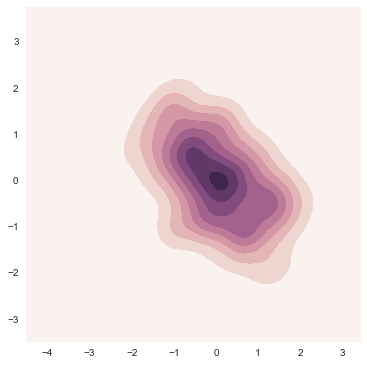
\includegraphics[width=0.7\linewidth]{images/color_palettes_40_0}
	\end{figure}
	
\end{frame}
%====================================%
\begin{frame}[fragile]
	\frametitle{Seaborn Workshop}
	\large
	\begin{itemize}
		\item To help select good palettes or colormaps using this system, you can use the \texttt{choose\_cubehelix\_palette()} function in a notebook to launch an interactive app that will let you play with the different parameters. 
		\item Pass \texttt{as\_cmap=True} if you want the function to return a colormap (rather than a list) for use in function like hexbin.
	\end{itemize}
	
\end{frame}
\section{Custom sequential palettes with \texttt{light\_palette()} and \texttt{dark\_palette()}}
%====================================%
\begin{frame}[fragile]
	\frametitle{Seaborn Workshop}
	\large
	\begin{itemize}
		\item For a simpler interface to custom sequential palettes, you can use \texttt{light\_palette()} or \texttt{dark\_palette()}, which are both seeded with a single color and produce a palette that ramps either from light or dark desaturated values to that color. 
		\item These functions are also accompanied by the \texttt{choose\_light\_palette()} and \texttt{choose\_dark\_palette()} functions that launch interactive widgets to create these palettes.
	\end{itemize}
	
\end{frame}
%====================================%
\begin{frame}[fragile]
	\frametitle{Seaborn Workshop}
	\large
	\begin{verbatim}
	sns.palplot(sns.light_palette("green"))
	\end{verbatim}
	
	\begin{figure}
		\centering
		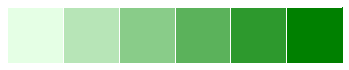
\includegraphics[width=0.7\linewidth]{images/color_palettes_43_0}
		\caption{}
		\label{fig:color_palettes_43_0}
	\end{figure}
	
\end{frame}
%====================================%
\begin{frame}[fragile]
	\frametitle{Seaborn Workshop}
	\large
	\begin{verbatim}
	sns.palplot(sns.dark_palette("purple"))
	\end{verbatim}	
	
	
	\begin{figure}
		\centering
		
\includegraphics[width=0.7\linewidth]{images/color_palettes_44_0}
		\caption{}
		\label{fig:color_palettes_44_0}
	\end{figure}
	
\end{frame}
%====================================%
\begin{frame}[fragile]
	\frametitle{Seaborn Workshop}
	\large
	These palettes can also be reversed.
	\begin{verbatim}
	sns.palplot(sns.light_palette("navy", reverse=True))
	\end{verbatim}
	\begin{figure}
		\centering
		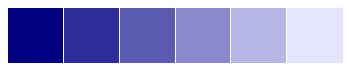
\includegraphics[width=0.7\linewidth]{images/color_palettes_46_0}
		\caption{}
		\label{fig:color_palettes_46_0}
	\end{figure}
	
	
\end{frame}
%====================================%
\begin{frame}[fragile]
	\frametitle{Seaborn Workshop}
	\large
	
	They can also be used to create colormap objects rather than lists of colors.
	\begin{verbatim}
	pal = sns.dark_palette("palegreen", as_cmap=True)
	sns.kdeplot(x, y, cmap=pal);
	\end{verbatim}
	
	\begin{figure}
		\centering
		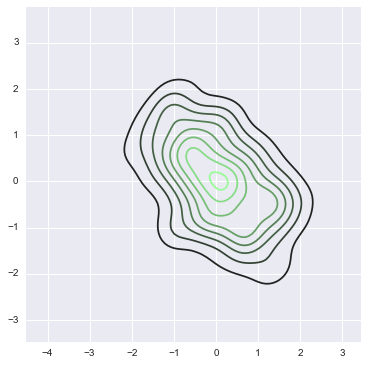
\includegraphics[width=0.7\linewidth]{images/color_palettes_48_0}
		\caption{}
		\label{fig:color_palettes_48_0}
	\end{figure}
\end{frame}
%====================================%
\begin{frame}[fragile]
	\frametitle{Seaborn Workshop}
	\large
	\begin{itemize}
		\item
		By default, the input can be any valid matplotlib color. 
		\item Alternate interpretations are controlled by the input argument.
		\item  Currently you can provide tuples in hls or husl space along with the default rgb, and you can also seed the palette with any valid xkcd color.
	\end{itemize}
\end{frame}
%====================================%
\begin{frame}[fragile]
	\frametitle{Seaborn Workshop}
	\large
	\begin{verbatim}
	sns.palplot(sns.light_palette((210, 90, 60), input="husl"))
	\end{verbatim}
	\begin{figure}
		\centering
		
\includegraphics[width=0.7\linewidth]{images/color_palettes_50_0}
		\caption{}
		\label{fig:color_palettes_50_0}
	\end{figure}
	
\end{frame}
%====================================%
\begin{frame}[fragile]
	\frametitle{Seaborn Workshop}
	\large
	\begin{verbatim}
	sns.palplot(sns.dark_palette("muted purple", input="xkcd"))
	\end{verbatim}
	\begin{figure}
		\centering
		
\includegraphics[width=0.7\linewidth]{images/color_palettes_51_0}
	\end{figure}
	
	Note that the default input space for the interactive palette widgets is husl, which is different from the default for the function itself, but much more useful in this context.
\end{frame}
%=================================================================== %
\section{Diverging color palettes}
%====================================%
\begin{frame}[fragile]
	\frametitle{Seaborn Workshop}
	\large
	
	\noindent \textbf{Diverging color palettes}
	\begin{itemize}
		\item The third class of color palettes is called “diverging”. These are used for data where both large low and high values are interesting. 
		\item There is also usually a well-defined midpoint in the data. 
		\item For instance, if you are plotting changes in temperature from some baseline timepoint, it is best to use a diverging colormap to show areas with relative decreases and areas with relative increases.
	\end{itemize}
\end{frame}
%====================================%
\begin{frame}[fragile]
	\frametitle{Seaborn Workshop}
	\large
	\begin{itemize}
		\item The rules for choosing good diverging palettes are similar to good sequential palettes, except now you want to have two relatively subtle hue shifts from distinct starting hues that meet in an under-emphasized color at the midpoint. \item It’s also important that the starting values are of similar brightness and saturation.
	\end{itemize}
\end{frame}
%====================================%
\begin{frame}[fragile]
	\frametitle{Seaborn Workshop}
	\large
	\begin{itemize}
		\item It’s also important to emphasize here that using red and green should be avoided, as a substantial population of potential viewers will be unable to distinguish them.
		\item 
		It should not surprise you that the \textbf{\textit{Color Brewer}} library comes with a set of well-choosen diverging colormaps.
	\end{itemize}
	
\end{frame}
%====================================%
\begin{frame}[fragile]
	\frametitle{Seaborn Workshop}
	\large
	\begin{verbatim}
	sns.palplot(sns.color_palette("BrBG", 7))
	\end{verbatim}
	
	\begin{figure}
		\centering
		
\includegraphics[width=0.7\linewidth]{images/color_palettes_54_0}
		
	\end{figure}
	
	\begin{verbatim}
	sns.palplot(sns.color_palette("RdBu_r", 7))
	\end{verbatim}
	\begin{figure}
		\centering
		
\includegraphics[width=0.7\linewidth]{images/color_palettes_55_0}
	\end{figure}
	
\end{frame}
%====================================%
\begin{frame}[fragile]
	\frametitle{Seaborn Workshop}
	\large
	
	
	Another good choice that is built into matplotlib is the coolwarm palette. Note that this colormap has less contrast between the middle values and the extremes.
\end{frame}
%====================================%
\begin{frame}[fragile]
	\frametitle{Seaborn Workshop}
	\large
	
	\begin{verbatim}
	sns.palplot(sns.color_palette("coolwarm", 7))
	\end{verbatim}
	
	\begin{figure}
		\centering
		
\includegraphics[width=0.7\linewidth]{images/color_palettes_57_0}
	\end{figure}
	
	
\end{frame}
%====================================%
\section{Custom diverging palettes with \texttt{diverging\_palette()}}
\begin{frame}[fragile]
	\frametitle{Seaborn Workshop}
	\large
	
	\begin{itemize}
		\item You can also use the seaborn function \texttt{diverging\_palette()} to create a custom colormap for diverging data. (Naturally there is also a companion interactive widget, \texttt{choose\_diverging\_palette()}). This function makes diverging palettes using the husl color system. 
		\item You pass it two hues (in degreees) and, optionally, the lightness and saturation values for the extremes. 
		\item Using husl means that the extreme values, and the resulting ramps to the midpoint, will be well-balanced
		
	\end{itemize}
\end{frame}
%====================================%
\begin{frame}[fragile]
	\frametitle{Seaborn Workshop}
	\large
	\begin{verbatim}
	sns.palplot(sns.diverging_palette(220, 20, n=7))
	\end{verbatim}
	
	\begin{figure}
		\centering
		
\includegraphics[width=0.7\linewidth]{images/color_palettes_59_0}
	\end{figure}
	
	
	
	\begin{verbatim}
	sns.palplot(sns.diverging_palette(145, 280, 
	s=85, l=25, n=7))
	\end{verbatim}
	
	\begin{figure}
		\centering
		
\includegraphics[width=0.7\linewidth]{images/color_palettes_60_0}
	\end{figure}
\end{frame}
%====================================%
\begin{frame}[fragile]
	\frametitle{Seaborn Workshop}
	\large
	
	
	The sep argument controls the width of the separation between the two ramps in the middle region of the palette.
	\begin{verbatim}
	sns.palplot(sns.diverging_palette(10, 220, sep=80, n=7))
	\end{verbatim}
	
	\begin{figure}
		\centering
		
\includegraphics[width=0.7\linewidth]{images/color_palettes_62_0}
	\end{figure}
\end{frame}
%====================================%
\begin{frame}[fragile]
	\frametitle{Seaborn Workshop}
	\large
	It’s also possible to make a palette with the midpoint is dark rather than light.
	\begin{verbatim}
	sns.palplot(sns.diverging_palette(255, 133, 
	l=60, n=7, center="dark"))
	\end{verbatim}
	
	\begin{figure}
		\centering
		
\includegraphics[width=0.7\linewidth]{images/color_palettes_64_0}
	\end{figure}
	
\end{frame}
\section{Changing default palettes with set\_palette()}
%====================================%
\begin{frame}[fragile]
	\frametitle{Seaborn Workshop}
	\large
	\begin{itemize}
		\item The \texttt{color\_palette()} function has a companion called \texttt{set\_palette()}. 
		\item The relationship between them is similar to the pairs covered in the aesthetics tutorial. 
		\item \texttt{set\_palette()} accepts the same arguments as \texttt{color\_palette()}, but it changes the default matplotlib parameters so that the palette is used for all plots.
	\end{itemize}
	
\end{frame}
%====================================%
\begin{frame}[fragile]
	\frametitle{Seaborn Workshop}
	\Large
	\begin{framed}
		\begin{verbatim}
		def sinplot(flip=1):
		x = np.linspace(0, 14, 100)
		for i in range(1, 7):
		y = np.sin(x + i * .5) * (7 - i)
		plt.plot(x, y * flip)
		sns.set_palette("husl")
		sinplot()
		\end{verbatim}
	\end{framed}
	
\end{frame}
%====================================%
\begin{frame}[fragile]
	\frametitle{Seaborn Workshop}
	\large
	
	
	\begin{figure}
		\centering
		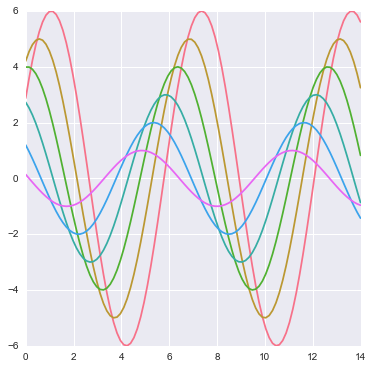
\includegraphics[width=0.7\linewidth]{images/color_palettes_67_0}
	\end{figure}
	
\end{frame}
%====================================%
\begin{frame}[fragile]
	\frametitle{Seaborn Workshop}
	\large
	\begin{itemize}
		\item The \texttt{color\_palette()} function can also be used in a with statement to temporarily change the color palette.
	\end{itemize}
	\begin{verbatim}
	
	with sns.color_palette("PuBuGn_d"):
	sinplot()
	\end{verbatim}
	
	\begin{figure}
		\centering
		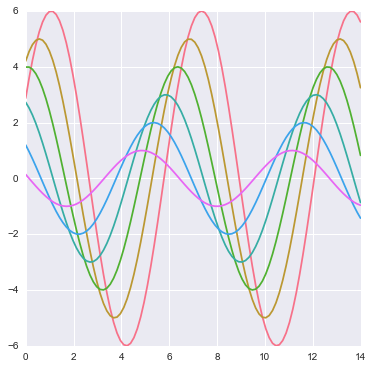
\includegraphics[width=0.7\linewidth]{images/color_palettes_67_0}
	\end{figure}.png
\end{frame}
%====================================%

\end{document}
